\documentclass{jsarticle}
\title{平成\ThisYrJP(\ThisYr)年度カタクチイワシ対馬暖流系群の資源評価}
\author{}
\date{}

\newcommand{\ThisYr}{2018}
\newcommand{\ThisYrJP}{30}

\begin{document}
\maketitle
\section{まえがき}
\section{生態}
\section{漁業の状況}
\section{資源の状態}
\section{\ThisYr 年ABCの算定}
\section{ABC以外の管理方策の提言}

\begin{figure}[htp]
 \begin{minipage}{0.5\hsize}
  \begin{center}
   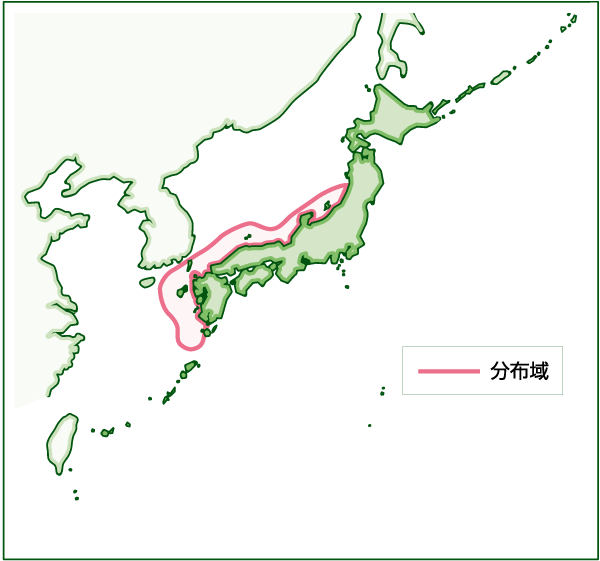
\includegraphics[width=70mm]{figs/map.png}
  \end{center}
  \caption{カタクチイワシ対馬暖流系群の分布域}
  \label{fig:distrib}
 \end{minipage}
 \begin{minipage}{0.5\hsize}
  \begin{center}
   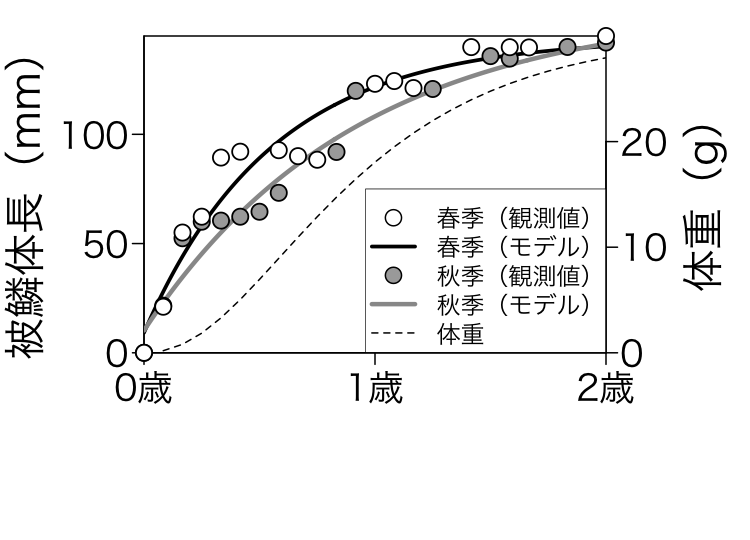
\includegraphics[width=70mm]{figs/age_length.png}
  \end{center}
  \caption{カタクチイワシの成長様式}
  \label{fig:agelen}
 \end{minipage}
\end{figure}

\end{document}
